
\section{Rodzaje fal sprężystych}
\label{sec:rodzaje_fal_sprezystych}

\subsection{Fale podłużne}

\begin{equation}
c_L=\sqrt{\frac{\lambda+2\mu}{\rho}}
\end{equation}
gdzie
\begin{eqwhere}[2cm]
        \item[$c_L$] prędkość fali podłużnej
        \item[$\lambda, \mu$] stałe Lam\'{e}go
        \item[$\rho$] gęstość ośrodka
\end{eqwhere}

\begin{figure}[h]
\centering
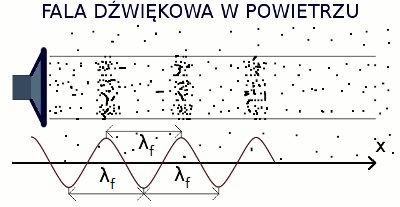
\includegraphics[width=10cm]{Zdjecia/2/fala_podluzna}
\caption{Przykład fali podłużnej}
\label{fig:fala_podluzna}
\end{figure}



\begin{figure}[h]
        \centering
        \begin{subfigure}{0.35\textwidth}
                \centering
	     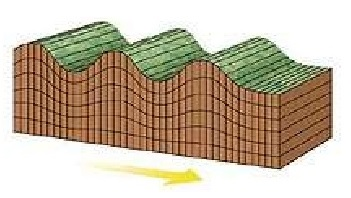
\includegraphics[width=5cm]{Zdjecia/2/fala_rayleigha}
                \subcaption{\label{subfigure_a}}
        \end{subfigure}
        \begin{subfigure}{0.35\textwidth}
                \centering
	     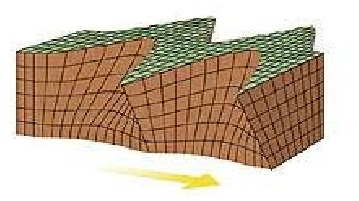
\includegraphics[width=5cm]{Zdjecia/2/fala_lova}
                \subcaption{\label{subfigure_b}}
        \end{subfigure}
        \label{fig:subcaption_example}
        \caption{Fale powierzchniowe: \protect\subref{subfigure_a} fala Rayleigha, \protect\subref{subfigure_b} fala L\"{o}va}
\end{figure}





















